\clearpage
\section*{S18. Expanded receiver and sharp-interface stress evidence}
\subsection*{Receiver Geometry and Calibration as Design Conditions}

A current-bank correction reaches an experiment only through its observation factor \(Y_C=S\bar C\). In a far-field receiver, \(S\) is the transverse radiation operator, including phase and geometric amplitude. At a finite stand-off distance it is instead the full dyadic Green map. The retained feedback \(\bar C\), the material-injection factor \(N_C\), and the Schur matrix \(\Gamma_C\) are fixed when only the receiver changes. The observation factor changes directly with aperture and calibration. Although \(N_C\) itself remains fixed, its material lift \(M_0N_C^*\) can also change because the regularized normal inverse \(M_0\) depends on the receiver. This separation is a mathematical prerequisite for extending a Fresnel-aware, \(k\)-space electromagnetic imaging workflow toward calibrated multiple-scattering material updates. The authors' FAEMIS (Fresnel-Aware Electromagnetic Inverse Scattering) project already studies finite-range/array operator corrections, spectral preconditioning, and amplitude calibration [14, main manuscript], while its present forward/imaging baselines use Born-type linearization. Our receiver experiments do not reproduce that project or use hardware data; they isolate the additional full-wave material-update requirement.

Suppose the complex measurements have covariance \(\Gamma_n\succ0\), and a known, invertible calibration map \(T\) is applied coherently to predicted data, observations, and covariance. Then \(J'=TJ\), \(r'=Tr\), and \(\Gamma_n'=T\Gamma_nT^*\). Direct substitution gives
\begin{equation}
J'^*\Gamma_n'^{-1}J'=J^*\Gamma_n^{-1}J,\qquad
J'^*\Gamma_n'^{-1}r'=J^*\Gamma_n^{-1}r.
\tag{S15}\label{eq:calibration-invariance}
\end{equation}
A known invertible amplitude/phase recalibration therefore changes coordinates, not the regularized local material step. An image-domain amplitude correction fitted using the true material is a different, oracle operation and cannot establish this invariance for an unknown target.

The same algebra preserves the paired material space itself. For the fixed current bank, \(Y_C'=TY_C\), while \(N_C\) and \(\Gamma_C\) are unchanged. Because \(J_0'^*\Gamma_n'^{-1}Y_C'=J_0^*\Gamma_n^{-1}Y_C\), the noise-weighted reduced normal inverse \(M_0\) and both generators of \(\mathcal E_0(C)\) are identical. Thus an exactly known, invertible receiver recalibration cannot by itself improve or degrade the specified-bank material-update closure. This conclusion fails for a singular aperture mask or for a gain map applied without transforming the corresponding noise model.

By contrast, discarding receiver components is a noninvertible change of experiment. For a correctly marginalized observation mask \(P\), define the whitened information matrix \(F_P=J^*P^*(P\Gamma_nP^*)^{-1}PJ\). Then \(F_P\preceq F=J^*\Gamma_n^{-1}J\): the omitted data cannot increase Fisher information for a fixed physical Jacobian. This order does not imply that a particular paired correction always shrinks monotonically, because the candidate bank, residual, and regularized optimization geometry also enter its gain. The quantity \(\sigma_{\min}(\Gamma_n^{-1/2}Y_C)\) on a declared observation subspace, together with the corresponding material injection \(N_C\), makes the design condition testable.

A sensitivity loss is not by itself a reconstruction-error lower bound. Let \(\mathcal A\) be the declared admissible material set and let \(\eta\) bound noise in the whitened receive norm. If two states \(\chi_1,\chi_2\in\mathcal A\) have \(\|\Gamma_n^{-1/2}[F(\chi_1)-F(\chi_2)]\|\le2\eta\), their noise balls intersect. Any estimator given an observation in that intersection has worst-case physical-material error at least \(\|\chi_1-\chi_2\|_{M_\chi}/2\). This is a conditional two-point bound for the specified forward model, admissible set, and error budget; finite-amplitude use requires both full-wave responses, not just a local singular value. A calibration-error set can be included by enlarging the two receive-data sets before testing intersection.

Our operator check compares complete dyadic receivers at radii 5, 10, and 20 with a phase- and amplitude-matched strict far-field map. At a saved \(12^3\) voxel iterate for the sharp sphere target, the relative full-wave current-response differences are 8.29\%, 4.14\%, and 2.07\%; at a saved \(12^3\) smooth-target Gaussian iterate they are 20.90\%, 10.31\%, and 5.14\%. In both cases the material state, incident fields, current basis, and candidate bank are frozen as the receiver moves. A known invertible gain/phase transformation preserves the tested whitened normal scalar and gradient to approximately \(10^{-15}\), whereas retaining every other receiver yields about half the information along one predeclared material probe. A separate small-model full-matrix check verifies the calibration identity and positive-semidefinite information loss to roundoff. The voxel case also shows why a raw lifted-signature norm is not an information score: the unwhitened \(\|M_0N_C^*\|_F\) rises from 848 to 1529 as the radius grows from 5 to 20, even while the fixed material probe's received sensitivity falls. The receiver-dependent inverse \(M_0\) changes the lift's scaling. These are synthetic Maxwell operator tests, not hardware measurements or complete inverse reconstructions.

To connect receiver choice to optimization, we also evaluated the paired and equal-real-rank Krylov corrections for one fixed material probe and one fixed absolute complex-noise realization at each of these two saved states. The residual is generated from that probe and the corresponding full receiver Jacobian; it is not an observed target residual. Figure~\ref{fig:faemis-repair} shows the same-radius far/finite paired-gain ratio and the within-receiver paired/Krylov gain ratio. Krylov gives larger full-quadratic gain in all 12 correlated receiver/state conditions. For the sharp-sphere iterate, replacing a finite receiver by its strict far-field approximation increases the paired gain by 2.2--4.3\% across the three radii; for the Gaussian iterate it decreases gain by 5.6--7.0\%. Thus a far-field approximation has no state-independent sign on the gain of this specified repair, even when its complex-field discrepancy decreases with distance. At fixed absolute noise, moving either receiver outward lowers the absolute paired gain, but cross-radius gains are different quadratic objectives and do not quantify reconstruction error. Supplement S12 records the individual values.

\begin{figure*}[tbp]\centering
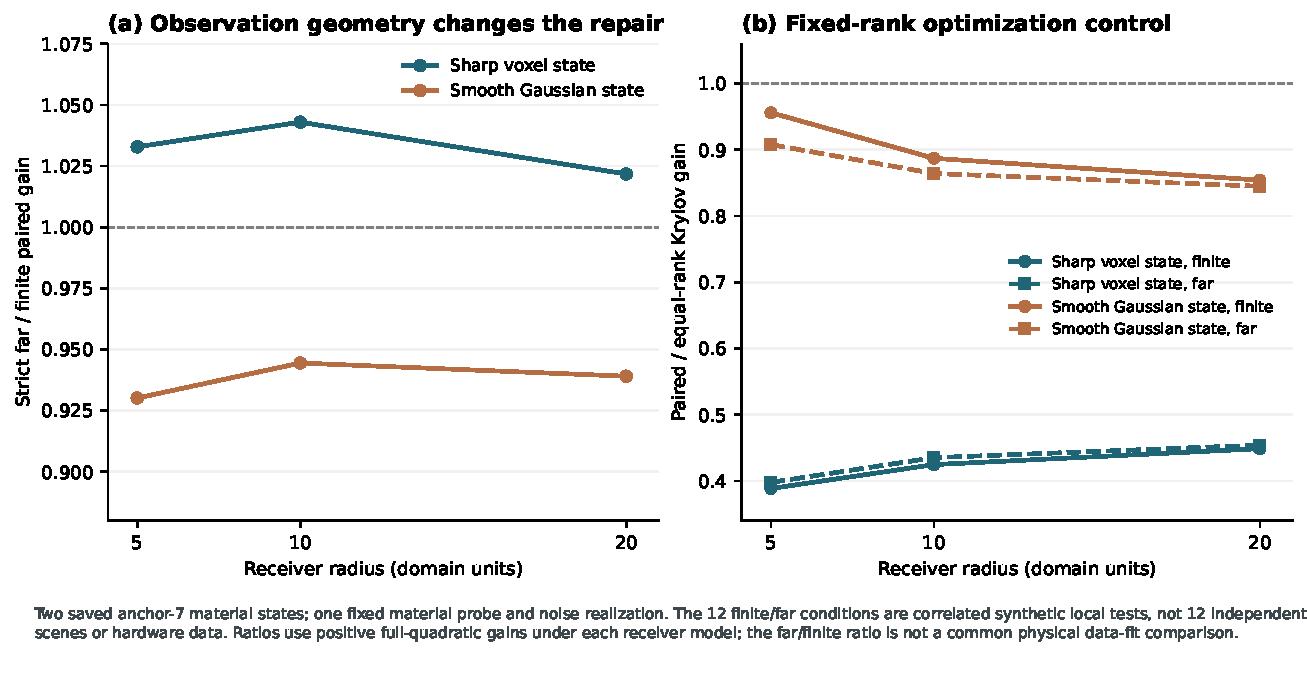
\includegraphics[width=0.96\textwidth]{figures/Figure_faemis_repair.pdf}
\caption{Receiver-dependent material-repair gains at two saved anchor-7 material states. (a) Strict-far paired gain divided by finite-receiver paired gain at the same radius. (b) Paired gain divided by equal-real-rank (48) material Krylov gain within each receiver and its own full local quadratic. The probe and absolute complex-noise realization are fixed per state; the residuals are synthetic. The 12 finite/far receiver/state conditions are correlated local tests, not independent scenes, hardware measurements, or reconstruction-error comparisons.}
\label{fig:faemis-repair}
\end{figure*}

\begin{figure}[tbp]\centering
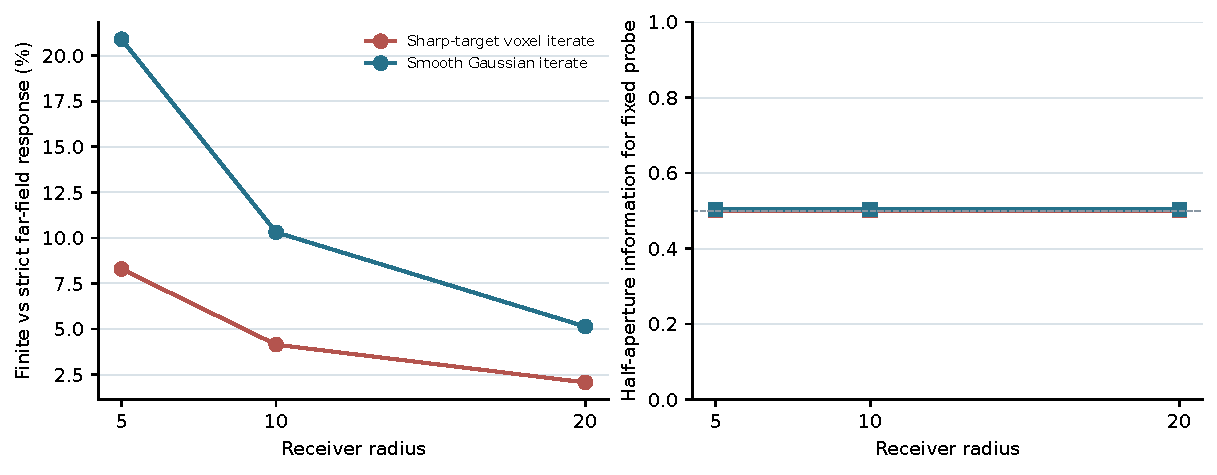
\includegraphics[width=0.98\columnwidth]{figures/Figure_farfield_aperture.pdf}
\caption{Synthetic receiver-design checks at two saved \(12^3\) material states. Radii 5, 10, and 20 use the same nondimensional length unit as the side-1.5 computational box and wavenumber 2.5. The strict far-field response is matched to each radius in propagation phase and \(1/r\) amplitude before taking a complex relative norm. Half-aperture information is one predeclared material-probe quadratic ratio, not a full-Jacobian singular-value or paired-repair bound.}
\end{figure}

\begin{figure}[tbp]\centering
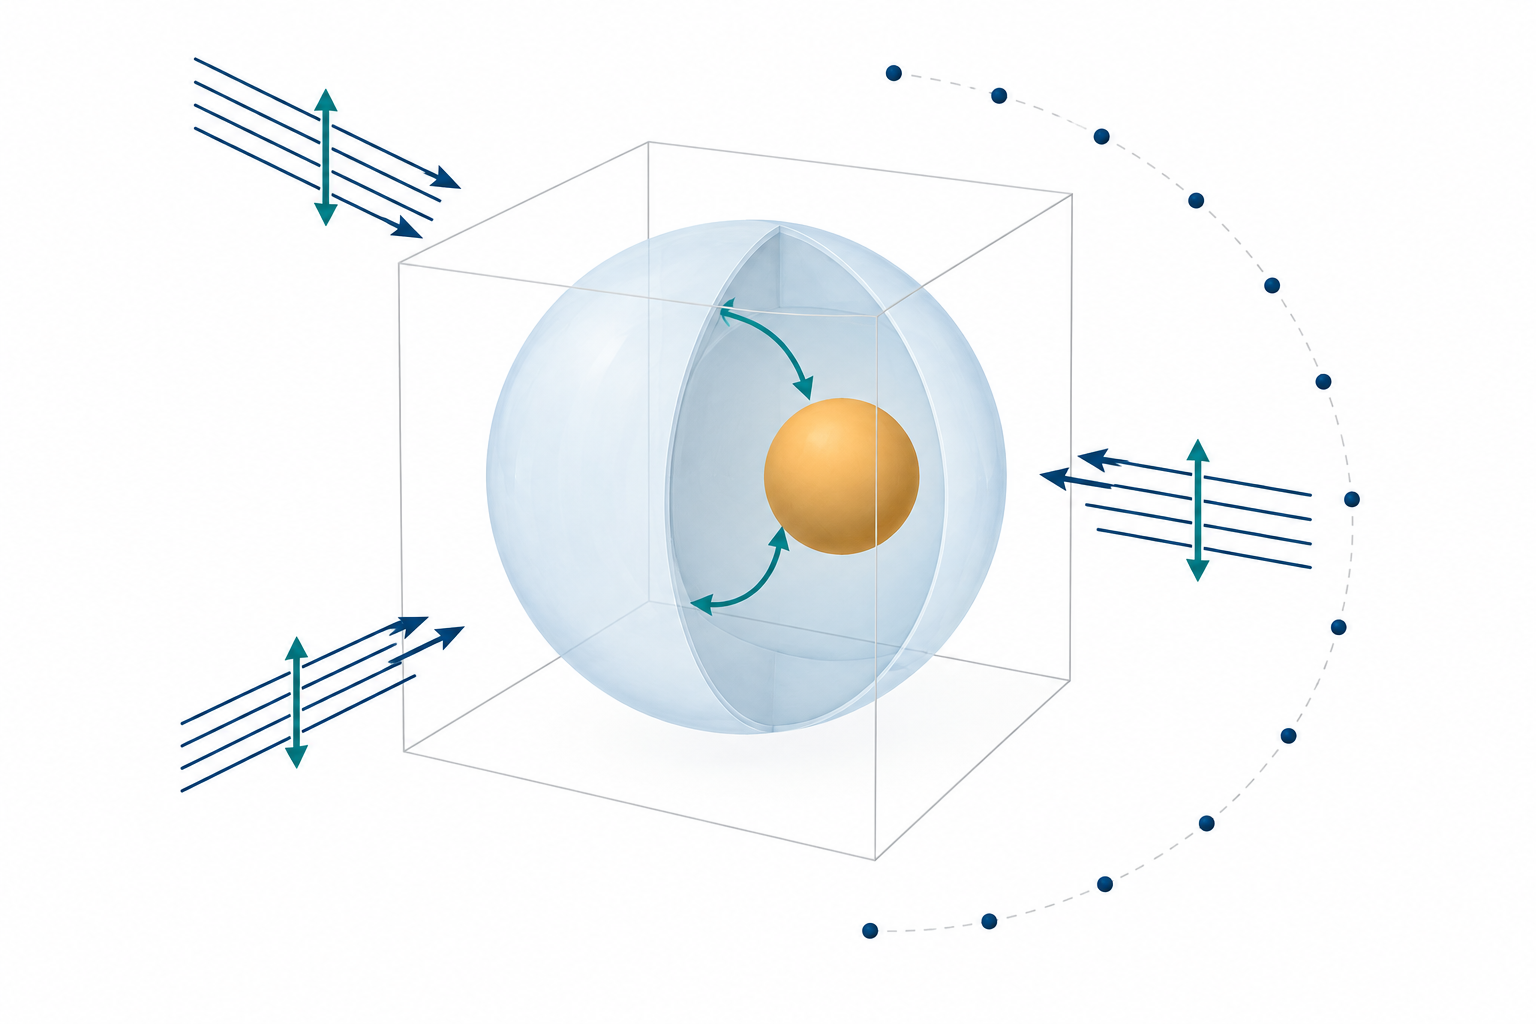
\includegraphics[width=0.96\columnwidth]{figures/scene_concept_3d.png}
\caption{Conceptual three-dimensional receiver scene: a sharply bounded dielectric object is illuminated from multiple directions, induces internal rescattering currents, and is observed in two transverse polarizations. The illustration describes acquisition geometry; it is not a computed field, reconstruction, or experimental datum.}
\end{figure}

\subsection*{Sharp-Interface Vector-Maxwell Challenge}

The preceding mechanism tests used smooth targets, which do not probe interface recovery. We therefore froze four higher-contrast geometries before running a new campaign: a homogeneous sphere, a two-material split rectangular solid, an eccentric-core shell, and two separated dielectric ellipsoids. All are in a vacuum box of side 1.5 at wavenumber 2.5, with six incident fields and dual-polarization reception. The new comparison uses physically normalized voxel material coordinates without giving the inverse solver true boundaries or regions. Truth is generated on a \(14^3\) grid and fitted on a \(12^3\) grid, within the same discrete-dipole family; same-grid \(14^3\) checks are labeled separately. The full-model preconditioned-CG route and a fixed \emph{Gs24 spectral selection rule} share initial material, regularization, constraints, noise realization, and nonlinear acceptance rule. The latter uses fresh primal anchors and state-dependent operators at each iteration, not a stale physical state or immutable current basis. Neither route executes the paired material repair. The sharp-scene record is reported separately from the original 72 correlated smooth-state local comparisons.

At \(12^3\), complex voxel contrast has 3456 real coordinates but the six illuminations provide only \(6\times128=768\) complex, or 1536 real, receiver values. The local material Jacobian is necessarily rank deficient before prior information. A small measurement residual cannot therefore certify a sharp material interface; recovery must be judged against the declared prior and truth as a separate endpoint.

We first quantify the full-wave/Born response difference, because large dielectric contrast alone does not prove a large retained-feedback contribution. Reconstruction assessment then uses real and imaginary material error on a common physical grid, fixed-threshold interface overlap, class-average contrast, held-out receiver data, true nonlinear objective reduction, fallback counts, and total cost. Local current-bank comparisons at full-model iterates 0, 3, and 7 use that iterate's actual damping. This distinction matters: the previous local bank study fixed a diagnostic curvature and cannot stand in for the new nonlinear-state comparisons.

All 16 frozen primary trajectories completed. Table~\ref{tab:sharp-primary} reports the zero-noise endpoints; the 1\% complex-noise cases use the same noise realization for both methods. The full-model route has smaller material and held-out-field errors in six of eight method pairs, but this relative ordering does not amount to successful sharp-interface inversion. Across the eight full-model runs, the median final/initial true-objective ratio is 0.00229, and the median fallback count is 12.5; objective decrease is therefore substantial despite weak material recovery. For example, the homogeneous sphere reaches 2.73\% held-out response error while its complex material error remains 75.52\% and thresholded support overlap is only 2.63\%. Its recovered mean interior real contrast is 1.91 versus the specified 5.0. The two separated ellipsoids are not recovered by either route: support overlap is zero in both noise conditions, and the true real-contrast-7 class averages only 0.78 in the zero-noise full-model image. The shell is the best-recovered case by support overlap, about 69.25\% for the zero-noise full-model run, although its complex material error remains 56.03\% and the contrast-7 core averages 3.73. These are endpoint measurements against the specified discrete truth, not estimates of continuum material error.

\begin{table}[tbp]\centering\caption{Frozen sharp-interface primary endpoints at zero measurement noise. Material error is the relative complex contrast error; IoU is thresholded outer-support overlap; held-out error uses receiver data omitted from fitting. The last column is the full-model response difference from its first-Born counterpart at the true discrete material. Every row compares a full-model preconditioned-CG update (F) with a fixed current-space update (R), each after at most 18 accepted nonlinear iterations. The two routes have different accuracy, so their run times are not a matched-quality acceleration comparison.}\label{tab:sharp-primary}
\resizebox{\columnwidth}{!}{\begin{tabular}{lrrrrrrr}\hline
Target & Mat. F & Mat. R & IoU F & IoU R & Held-out F & Held-out R & Full/Born \\\hline
Sphere & .755 & .766 & .026 & .000 & .027 & .032 & .695\\
Split cuboid & .750 & .757 & .455 & .437 & .047 & .055 & .606\\
Eccentric shell & .560 & .587 & .692 & .675 & .019 & .026 & .736\\
Two ellipsoids & .906 & .901 & .000 & .000 & .073 & .072 & .335\\\hline
\end{tabular}}
\end{table}

The full/Born differences range from 33.5\% to 73.6\%. The separated ellipsoids have the highest constituent contrast but the smallest measured departure from Born in this set. Material contrast alone is therefore a poor proxy for the realized multiple-scattering strength under a given geometry and illumination. The fixed current-space route is sometimes faster in wall time, but it does not reach the same material or data endpoint in the six pairs where the full route wins. We accordingly do not infer an inverse-solver speedup from these unequal-quality runs.

At the saved full-model pre-update states 0, 3, and 7 for each zero-noise target, we also compared three specified current banks (residual, Gs, and TSOM-inspired) under the \emph{same full regularized local quadratic}, using the actual damping of that update. These bank labels identify candidate generators, not complete native SOM or TSOM algorithms. Across 36 correlated scene--state--bank rows, the paired material repair improves the specified direct current enlargement in 36/36, while equal-real-rank material Krylov improves the paired repair in 36/36. Both material banks have rank 48 in every comparison. The paired-gain median is \(2.81\times10^{-4}\), between the direct-enlargement median \(1.79\times10^{-5}\) and Krylov median \(5.18\times10^{-4}\); two direct enlargements even increase the full quadratic. The prescribed step change lies in the computed paired envelope to a median relative \(H\)-distance \(1.12\times10^{-11}\) (maximum \(3.14\times10^{-10}\)). These are local, highly correlated comparisons and do not represent paired nonlinear reconstruction trajectories. Their agreement with the original 72-comparison ordering supports the mechanism beyond smooth targets while retaining the negative equal-rank result. Supplement S11 lists every row and the associated absolute distances.

The retained feedback has appreciable size in these sharp states: in 16/36 banks its radiated norm exceeds that of the direct candidate current, with a maximum feedback/direct ratio of 11.20. The total dressed/direct output ratio has median 1.25 and maximum 11.25. Thus inspecting only the raw radiation of a proposed current can miss a larger retained-space-mediated output. The ratio is not a material information score, and it does not determine the objective gain without the injection side and current full defect.

\begin{figure*}[tbp]\centering
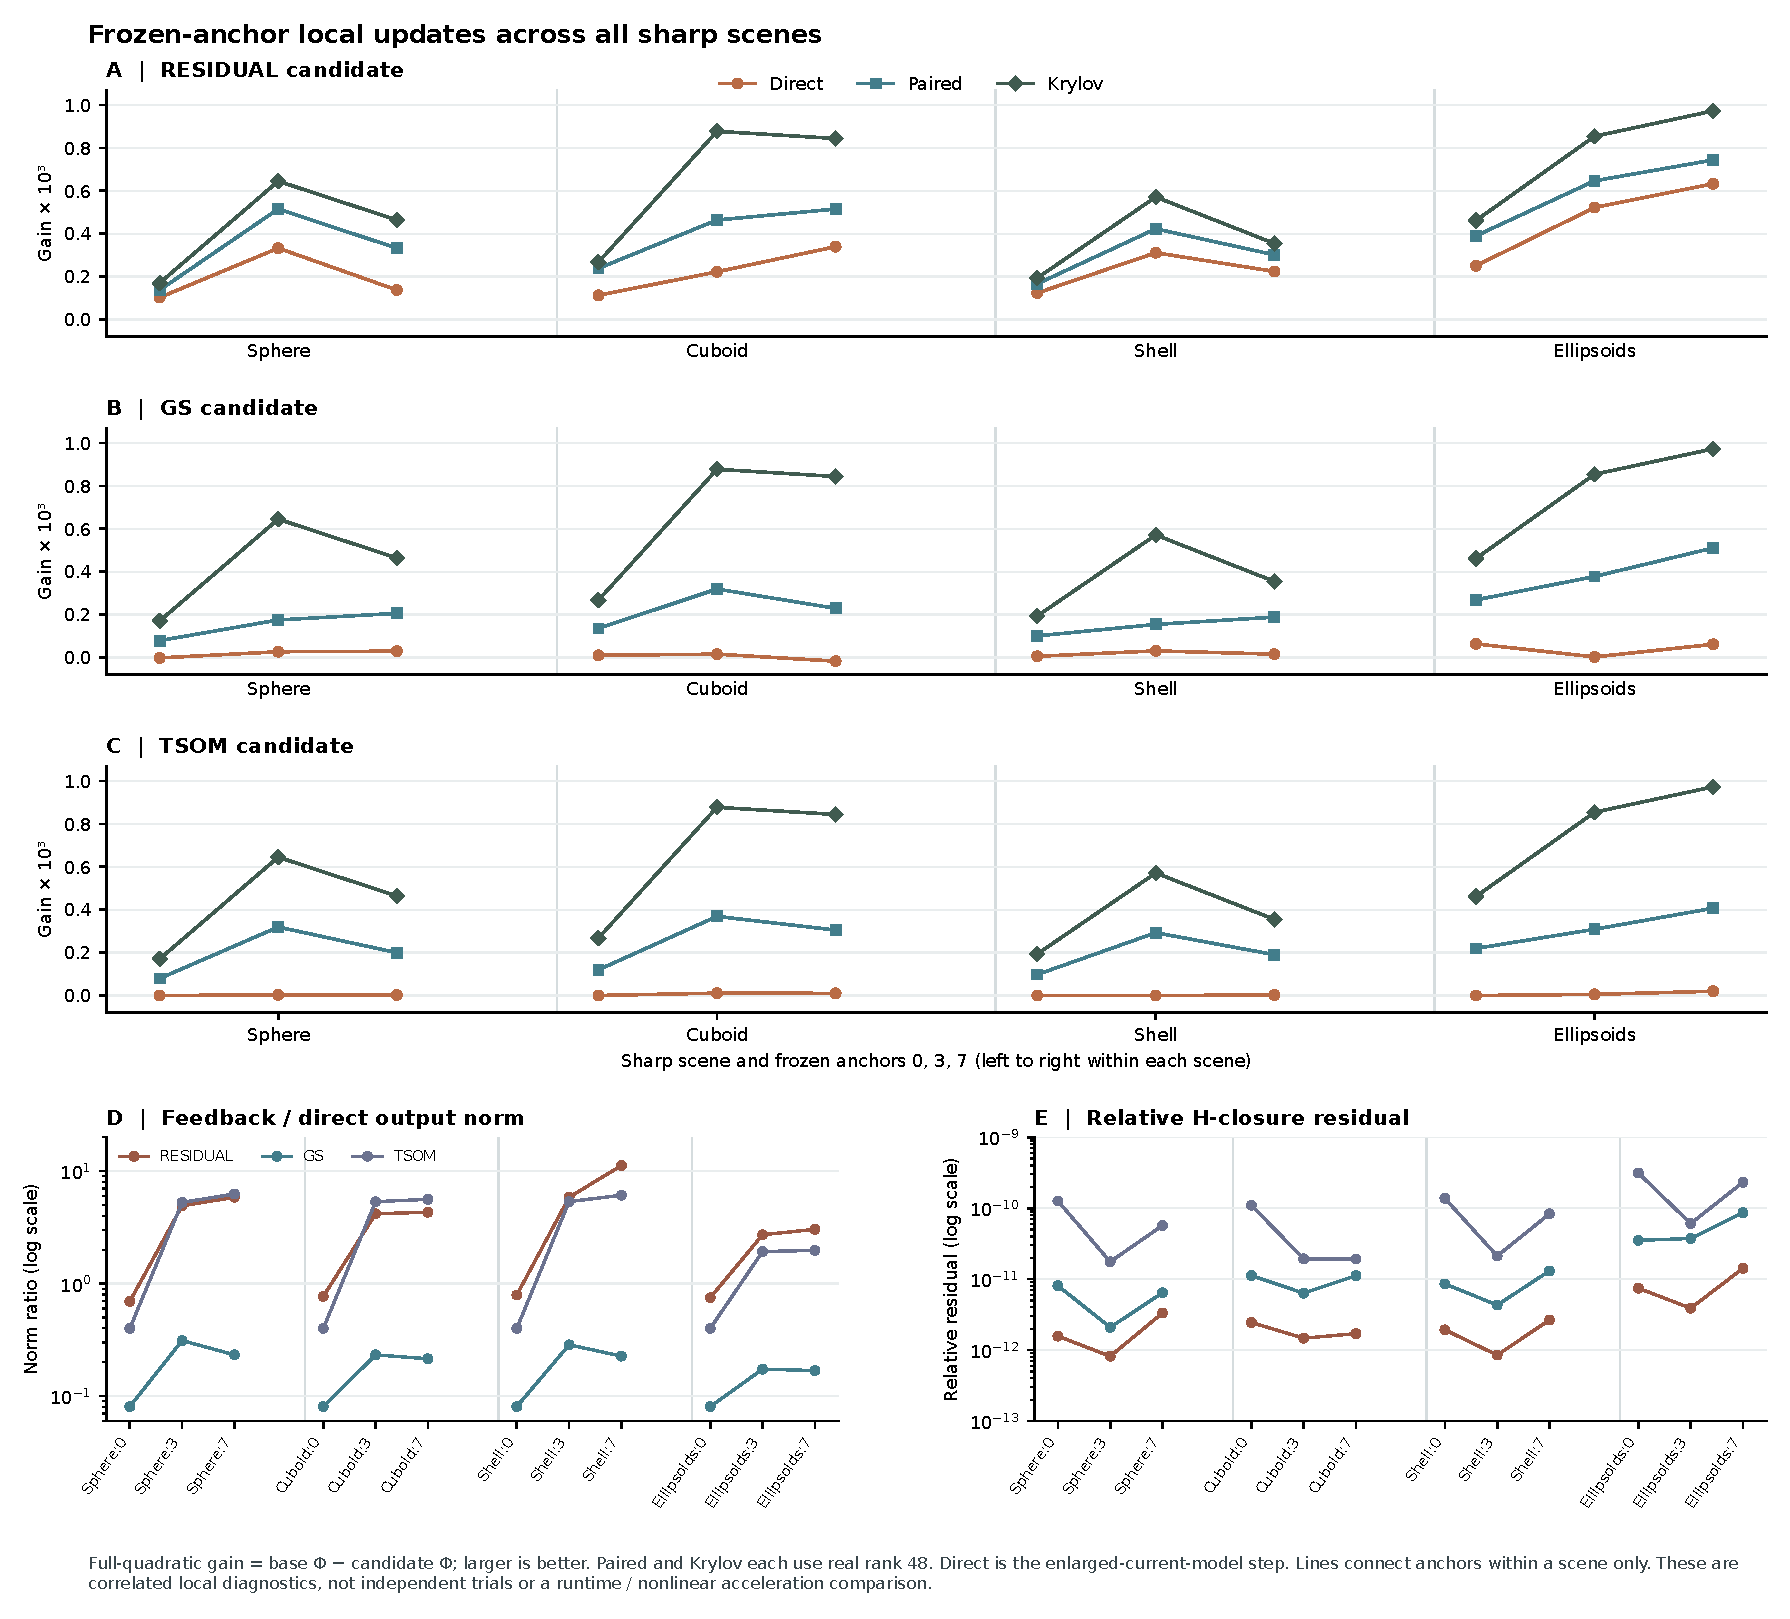
\includegraphics[width=0.96\textwidth]{figures/Figure_sharp_local.pdf}
\caption{Specified-bank local repair on four sharp vector-Maxwell targets. Three bank sources share each of 12 saved material states. The upper panels compare decrease in the same full regularized local quadratic for direct current enlargement, paired material repair, and equal-real-rank (48) material Krylov. The lower panels show retained-feedback/direct radiation and relative \(H\)-closure distance. All 36 rows are correlated frozen-state diagnostics rather than independent reconstructions; a negative direct gain is a worse full quadratic.}
\label{fig:sharp-local}
\end{figure*}

The predeclared 3\% noise extension covers only the split cuboid and eccentric shell, with a shared realization across the two methods. Full/fixed complex-material errors are 0.7501/0.7584 for the cuboid and 0.5830/0.5845 for the shell; corresponding held-out errors are 0.04666/0.05483 and 0.02454/0.02710. Material recovery remains limited, and the fixed shell route has slightly higher thresholded support overlap (0.6768 versus 0.6703). These four extension trajectories show that the primary negative material result is not confined to noiseless data, but do not establish general noise robustness.

The two predeclared same-grid \(14^3\) inverse-resolution pairs likewise do not resolve the material limitation. For the sphere, full/fixed complex-material errors are 0.7206/0.7366 and support overlaps are 0.0263/0; for the split cuboid, the corresponding values are 0.7153/0.7191 and 0.5980/0.5359. The cuboid boundary overlap improves relative to its \(12^3\) inversion, but its full-model held-out response error increases from 0.04655 to 0.05268. These same-family, same-grid runs are resolution checks, not independent continuum validation.

\begin{figure}[tbp]\centering
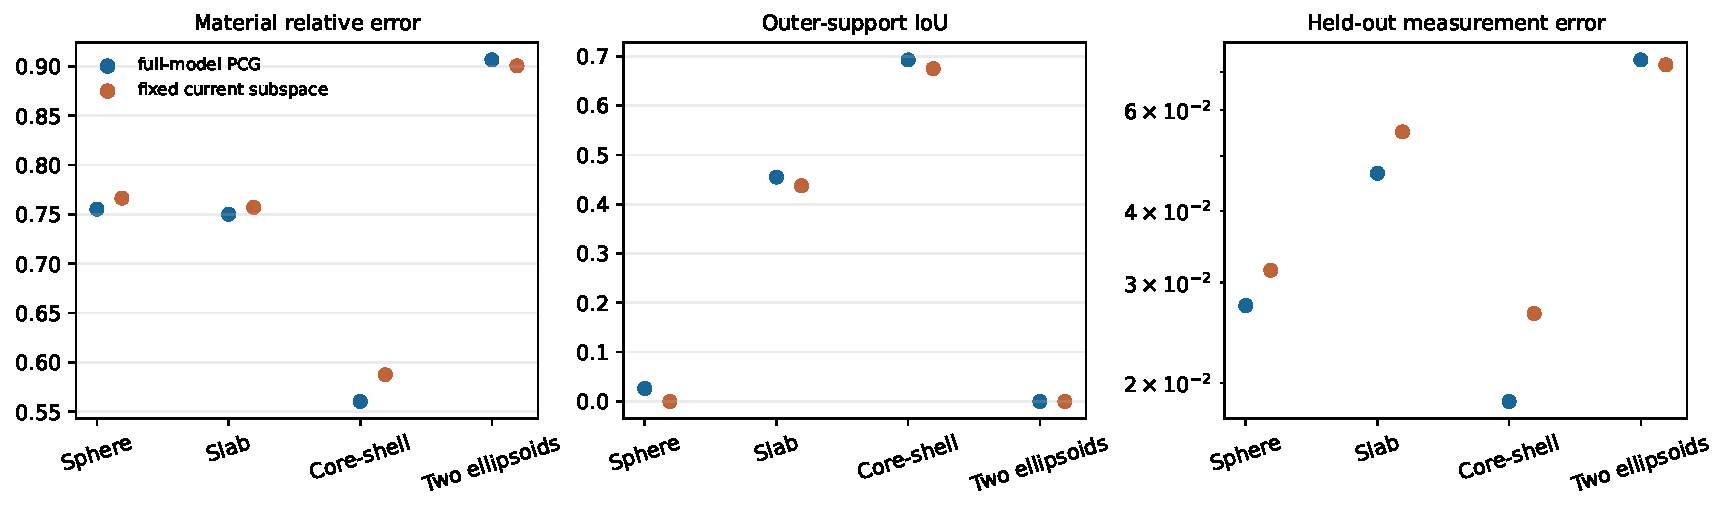
\includegraphics[width=0.98\columnwidth]{figures/Figure_sharp_primary_metrics.pdf}
\caption{Material error, held-out response error, and support overlap for the eight zero-noise trajectories in the 16-run primary campaign. Paired markers share the object, initialization, and acceptance rule. Small held-out response error can coexist with severe material and interface errors. The eight method pairs are correlated fixed scenarios, not a sample of 16 independent objects.}
\end{figure}

\begin{figure*}[tbp]\centering
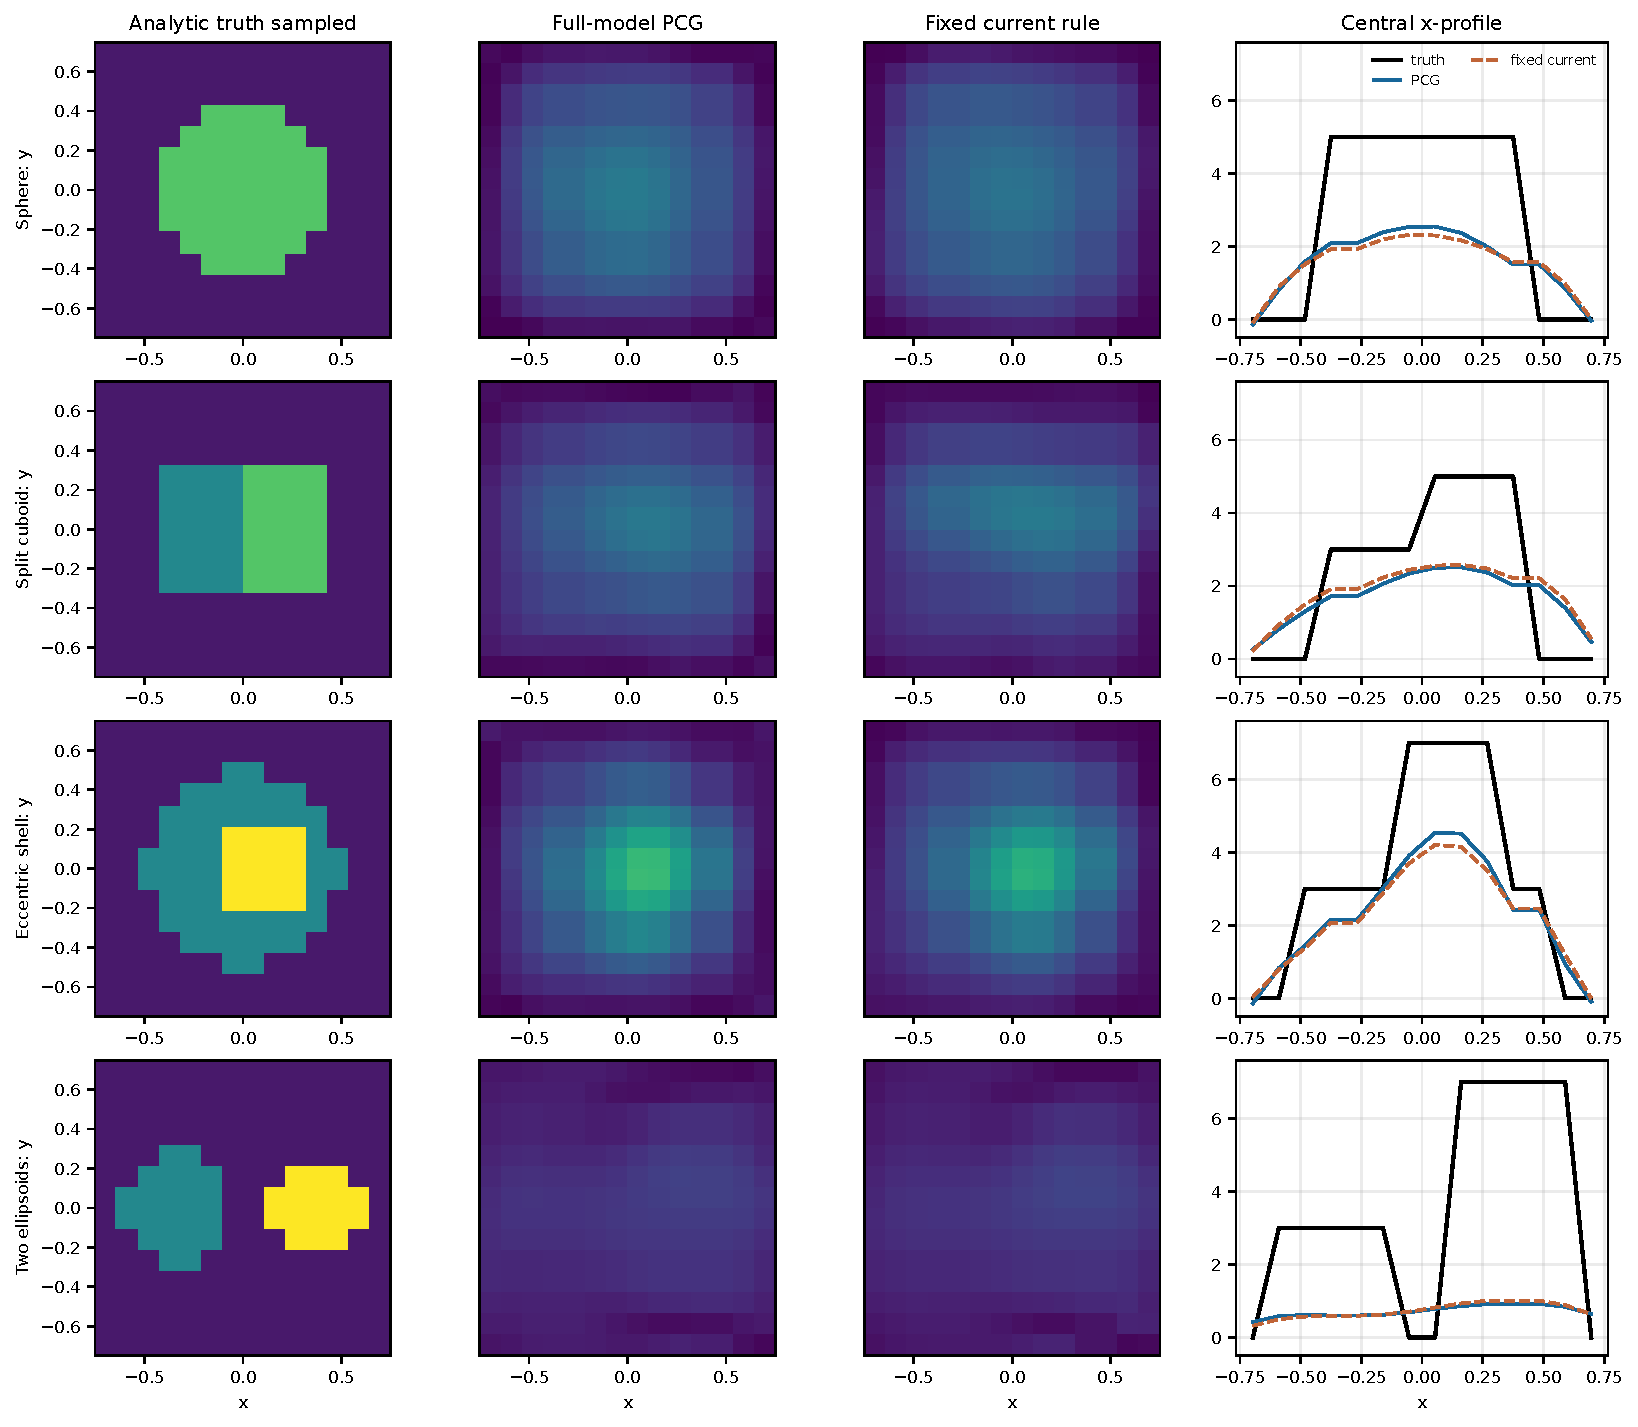
\includegraphics[width=0.96\textwidth]{figures/Figure_sharp_profiles.pdf}
\caption{Zero-noise real-contrast slices and central line profiles for all four frozen objects. The displayed truth is the analytic geometry sampled on the declared grid; reconstructions are mapped to that display grid with one common color scale. The full-model and fixed-current routes both smooth or miss sharp boundaries, particularly for the sphere and separated ellipsoids. This visualization supplements, rather than replaces, the complex-material and held-out-response metrics in Table~\ref{tab:sharp-primary}.}
\end{figure*}

An independent spherical-wave check places an important limit on the sharp-target validation. For the homogeneous sphere at contrast \(5+0.2i\), a predeclared forward receiver channel has complex-field relative errors of 21.40\% for the \(14^3\) DDA truth grid, 11.13\% at \(28^3\), and 9.73\% at \(32^3\), against the vector Mie series [15, main manuscript] after matching phase and far-field amplitude conventions. The finite voxel boundary makes convergence nonmonotone; this one-channel check is not a whole-aperture error bound. It nevertheless prevents interpreting the \(14^3\) same-family reference as a resolved continuum-Maxwell truth for this high-contrast sharp sphere. We keep material reconstruction and receiver-fit results relative to the declared discrete truth and do not transfer local ROM-step closure to continuum accuracy.

\begin{figure}[tbp]\centering
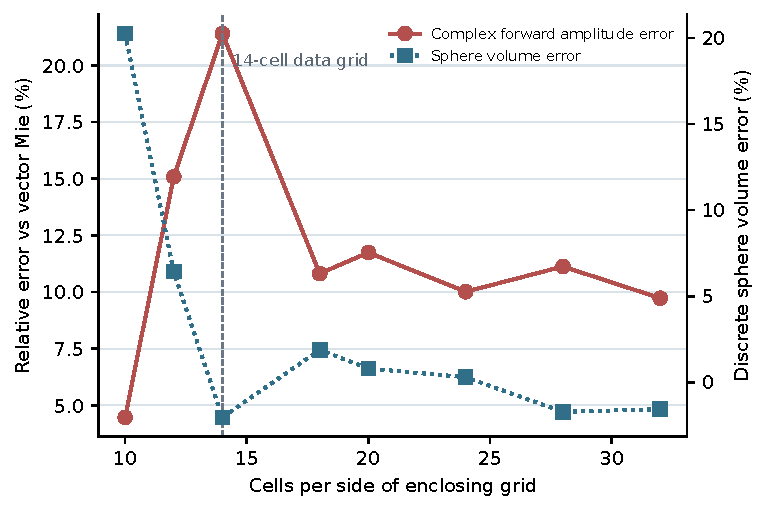
\includegraphics[width=0.98\columnwidth]{figures/Figure_mie_sharp_sphere.pdf}
\caption{Independent vector Mie comparison for one predeclared forward far-field channel of the high-contrast sphere. Complex-field errors are nonmonotone across voxel grids and remain 21.40\% at the \(14^3\) grid used to generate the main discrete truth. The plot is a forward-discretization diagnostic, not a bound for every receiver or a validation of recovered material.}
\end{figure}

